\chapter{Implementation}

% cleint handling
% server handling
% database/storage
% gesture recognition

% talk about actual implementation here. discuss controllers, how entities are stored.

% key data structures
% how are things stored
% what modules are available to the client and server
% where is the plugin architecture
% think of a picture

% how you write plugins. maybe show an example plugin (or snippet)

% "how do things work"

% 5 = architecture & implementation 
% 5.1 = key architectural design decisions
% 5.2 = implementation OR components


% - diagrams
% - expansion 
% -- plugin example (skeleton)
% - talk about input handling system (how i know what object you touch)
% - admin web server
% - "if this is what the screen looks like, then how are all the things stored"

\section{Networking}

\begin{figure}[htb]
  \centering
  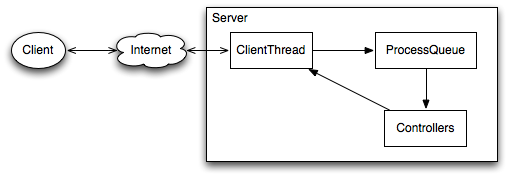
\includegraphics[width=0.8\textwidth]{network.png}
  \caption{Overview of Network Flow in Calico}
  \label{fig:network}
\end{figure}
% Intro parts
As a distributed and collaborative system, networking is a key part of Calico. The networking system must be able to support many clients at the same time, many of who may be working on the same workspace. The networking system in Calico consists of three major components: The main server socket and individual client process threads, the network queue processor, and the \texttt{CalicoPacket}. These three components work together to ensure that client requests are quickly handled, and that conflicts are properly managed.

% Socket/ClientThreads
The first component is the primary server socket and client threads. We decided to implement Calico as a TCP\cite{network} server in order to benefit from TCP's flow control and error correction. While TCP may be slower than UDP, the benefits of ensuring packets are received in the order they are sent as well as maintaining a continuous session outweighted any performance gains of UDP. When the Calico server is started, a TCP socket listener is created that waits for client connections to arrive. Upon receiving a new connection from a client, a new \texttt{ClientThread} is created that will then handle the connection with the client for the remainder of the client's session. By using a multi-threaded network system, we can easily maintain multiple sessions at the same time.

% ProcessQueue
The second component is the network queue processor, implemented as \texttt{ProcessQueue} class. This class is responsible for processing each packet that arrives from a client. When one of the \texttt{ClientThread}s receives a packet, the packet is then routed to the \texttt{ProcessQueue} which has a method for each packet type that can process that specific command. This class can then call any controllers as needed in order to complete the requested command.

% CalicoPacket
The \texttt{CalicoPacket} is responsible for encoding all information of a specific command into a byte array that can then be sent to clients. The packet is the lowest level of the networking system, but one of the most important. As noted in the previous section, the Calico packet was heavily based on Half-Life's network packet design. The first part of the packet contains a four-byte length which tells the system how far it needs to read in order to obtain the entire packet. By breaking commands down and transmitting them at the byte level, we were able to greatly reduce the network overhead that would be created if we had decided to send serialized objects over the network instead.


\section{Object Controllers}
In Calico the object controllers are responsible for handling all operations made on elements under their control. Each object type in Calico was provided with a controller.
Scraps, strokes, arrows, and canvases each have a controller that handles any interaction performed on the object. 
Controllers also act as the storage points for objects they are responsible for. This storage is discussed in the next section.

Controllers were created as static classes. This meant that each method in the controller would always be provided with the object's identifier, which it could then use to locate the object within the database. 
The controllers were also responsible for notifying the server of any changes that were performed. However, in order to prevent clients from sending notifications for actions that were not performed by the user, we created two types of functions for each action in the controller. The first function would perform the action and then notify the server, while a second function would perform the action without sending notifications. Any operation that was performed by the user would have a notification sent to the server. Any operation that was the result of receiving input from the server would not send a notification.


\section{Object Storage}
In Calico, all core components are stored using high performance Java hash maps. 
We decided that using FastUtil's\cite{fastutil} high performance maps would provide a better response time as opposed to using Java's core HashMap class. 
Each controller contains a single hash map that acts as a database for all objects that the controller is responsible for.
All access to hash maps requires use of a ``key'' to perform a lookup.
All objects are given a sequential 64-bit integer that acts as a globally unique identifier for each object.

One important design decision that was made was the choice to use a sequential identifier for each new object. The two factors that influenced our decision were: the relatively small size of a 64-bit integer in comparison with a universally unique string (which would be almost double the size), and better client performance.
Small size was very important to us - this identifier would be included in nearly every network packet that was sent to and from the server. We wanted the footprint to be as small as possible, but we needed something that we could ensure would be unique for every object. 
The second decision - better client performance - was another benefit provided by using a sequential identifier. Clients could request a pre-allocated block of identifiers that they could assign to objects created client-side. The client could then create objects and assign them an identifier and submit the object directly to the server. Due to the fact that identifiers were pre-allocated, the client did not have to wait for confirmation from the server in order to add the object to its local hash map.

\begin{figure}[htb]
  \centering
  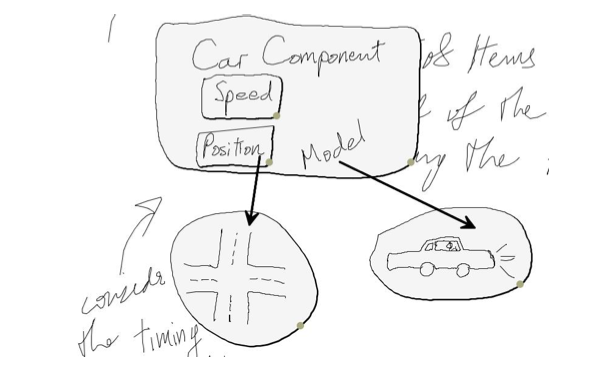
\includegraphics[width=0.8\textwidth]{scraps.png}
  \label{fig:scraps_storage}
\end{figure}

The screenshot shown above displays a typical design session in Calico. The content shown above would be stored in the various databases within each controller. This image represents a single \texttt{Canvas} object which would be stored within the \texttt{CanvasController} class. The \texttt{Canvas} object would have a list that contains the identifiers for each object that is being displayed on screen (five \texttt{Scrap}s, two \texttt{Arrow}s, and many \texttt{Stroke}s). Each of these objects would be stored in their respective controller. Each of these objects would require a list of \texttt{Point}s that would form the boundaries of the object. These are used within Calico to determine the location of an object, as well as whether an object is ``contained'' within another object (such as a scrap). Each object can have additional attributes that are specific to its type (arrows would need endpoints, strokes would have a color). These attributes would be stored within the object itself and would be converted to a \texttt{CalicoPacket} whenever a new client connected and needed to load the existing state of Calico.


\section{Plugin Framework}
To improve the extensibility of Calico, a plugin framework was created. This plugin framework allowed for extra features to be easily integrated into Calico. Plugins could subscribe to specific events that they wanted to be notified about. When one of these events was triggered within Calico, all subscribers to that event were notified, and could perform any action based upon the event information. 

\begin{figure}[htb]
  \centering
  \small
  \verbatiminput{figures/plugin.java}
  \normalsize
  \caption{Example plugin source code}
  \label{fig:plugin_file}
\end{figure}

To create a plugin, developers only had to extend a provided abstract plugin class that allowed each plugin to register itself with a \texttt{PluginManager} that was responsible for publishing network events and interface events to each plugin. Plugins were provided with default ``hooks'' that would be called upon when the plugin was loaded or unloaded. Plugins were able to call a method \texttt{registerNetworkCommandEvents} that would allow it to subscribe to specific network commands that it was interested in. Another method, \texttt{RegisterPluginEvent} enabled the plugin to subscribe to various interface events that could be used for processing user input and clicks. This plugin system provided a very easy way for developers to interact with the Calico framework, without needing to modify the code of the existing system. Developers could quickly create plugins that could interact with a live system.




\section{Input Handling}
% - talk about input handling system (how i know what object you touch)
% when the mouse pressed, locate all scraps that contain the mouse location
% determine the smallest scrap that contains the location
% actions are performed on that
% input handler is then "locked" onto that specific group (so that during the move, we are not trying to calculate over and over)
% unlocked as soon as it is released
% each object knows the list of points (or path) that acts as its bounds.
% Each object can then know if a specific point is within
In an effort to improve the user interaction experience, we felt that the existing input handling system needed to be created specifically for Calico. The previous version of Calico had relied on the input handler provided by the drawing framework that was used. This became unusable when working with canvases containing hundreds of objects. To improve response times, we need to recreate a newer input handler that did not rely on the drawing framework - meaning that it could continue to operate even while the drawing framework was busy rendering the display.

Rather than having a specific mouse listener linked to each object on screen, we instead decided to have a global mouse listener that could determine which object was being touched. This meant that mouse input only needed to be processed by a single handler, and based on various modes, it could intelligently handle interaction with the user. 

Each canvas maintained a list of all objects that were present on screen. Each object also was responsible for maintaining a list of coordinates that formed the ``bounds'' of that object. Objects could then easily determine if a specific point was contained with the ``bounds'' of that element.
Upon receiving any mouse input, the input handler would then iterate through the elements and determine which elements contained the mouse location. This list would then be further reduced to return only the \emph{smallest} object that contained the mouse location. This was very helpful when handling scraps that had been stacked on top of each other - the parent scrap still contains the mouse location, but clearly the user wants to interact with one of the child elements.

After locating the element that the user will be performing actions with, the input handler would then be ``locked'' to only interact with that element until the mouse has been released. This meant that users could move a scrap around screen (and move the mouse outside the bounds of the selected scrap) and still have the scrap follow the mouse location. Another benefit of locking the input handler on a specific element was that while doing very intensive operations (such as moving an element across the screen) we were not wasting resources to recalculate which element we were interacting with. This is something that was not availble in the previous versions of Calico.

The one drawback to using this approach meant that the object location and screen coordinate systems were identical. What that meant was that the Calico coordinate system was equal to the user's screen resolution. If a user with a larger screen joined the session, they could draw shapes and figures that were outside the viewable area of users with smaller screens. At the time, this was not a problem because all users were running the same resolution, so fortunately this problem rarely occurred.

\section{Administrative Interface}
% - admin web server
% uses httprequesthandlers
% velocity templates
% based off phpBB admin interface
% has a few basic functions, and allows admins to administer those
% view connected clients
% update configuration values
% upload images
% execute specific commands
% perform backup
% restore backups
One of the last components to be added was the administrative interface. Calico now had a headless server, and we needed a way to remotely manage it. We decided against building the interface within the Calico client - we wanted to keep the client as lightweight as possible. 
We decided to create an easy to use web-based interface that would allow the Calico server to be managed easily using a web browser.

To keep the admin system lightweight, we decided to just utilize simple \texttt{HttpRequestHandler}s that were tied to a single \texttt{HttpService} listening for web connections. All frontend HTML and CSS was generated using Velocity\cite{velocity} templates. The interface look-and-feel was copied from the administrative interface of an open-source forum system known as PhpBB\cite{todo}.

The administrative interface only provided basic management abilities. The core abilities it provided were:
\begin{itemize}\itemsep1pt

\item
\textbf{Easily modify settings}.
We needed the ability to modify the settings of an existing Calico instance easily. What was created was a page that listed all the configuration variables and easily let the administrator modify those values. When saved, the Calico server could then be restarted if needed to reflect the configuration changes.

\item
\textbf{View currently connected clients}. 
This was helpful in the classroom environment to be able to see all users who were currently connected to the server. In the future we planned to add the ability to ``kick'' clients from the server, but this was never full developed.

\item
\textbf{Perform backups and restoration of sessions}.
One of the major requirements was the ability to easily generate a backup of an entire session. Our goal was to provide an easily way to download a backup file that represented the current state of the server. It needed to contain all the data required to fully restore all canvases and any scraps, strokes, or arrows that may be contained in the canvas. Once we created the backup system, we needed a way for a server to restore any backup. Our administrative interface provided an easy to use form where a backup file could be selected and then uploaded directly to a running server. The server would then read the contents of this file and import all data into the server. Restoring a backup essentially wiped any existing content and recreated the entire session from scratch. Once a restoration had been performed, clients could reconnect and they would see all the data, just as it was when the backup was created.

\end{itemize}

These few requirements were the driving force behind the administrative interface. It stands as a very barebones and minimalistic interface that provides functions that we decided were essential to operation. This administrative interface has proved invaluable when generating and restoring backups. Having a backup of sessions provides users with a greater level of reassurance that any work they have made will not be lost should anything happen to the server.


